\section{Schumacher's Quantum Noiseless Channel Coding Theorem}

\subsection{Channel Compression}

\subsubsection{What is Channel Compression?}
Channel compression is the process of encoding information in a way that minimizes the required resources, like \textbf{bits} in Classical Channels or \textbf{qubits} in Quantum Channels. In this way, we can preserve the integrity of the original message during transmission across the channel. 

\subsubsection{Why Channel Compression?}
\begin{itemize}
    \item \textbf{Efficiency:} All communication channels, whether classical or quantum, have finite capacities. Compressing information ensures that these capacities are utilized effectively without wastage.
    \item \textbf{Adaptability to Noise:} By compressing and encoding the message efficiently, we can cut-down the effects of noise present in the channel, improving reliability of transmission in communication systems. 
\end{itemize}

\subsubsection{In the Classical Context}
In classical information theory, channel compression minimizes the number of bits needed to transmit a message over a channel without loss. These compression techniques are based on Shannon's Source Coding Theorem, which aim to achieve rates close to the source entropy \(H(X)\), where \(X\) represents the random variable describing the source in question. 

\subsubsection{In the Quantum Context}
Schumacher’s Compression Theorem provides a way to compress quantum information down to the von Neumann entropy, indicating the minimum qubits needed to achieve high-fidelity state reconstruction. Quantum (communication) systems are inherently fragile and resource-intensive. We reduce the physical and computational resources needed to transmit relevant quantum information. 

\subsection{Classical Compression - Shannon's Source Coding Theorem}

Shannon’s Source Coding Theorem establishes the minimum average number of bits needed to represent information from a classical source without loss, which is directly related to the entropy of the source.

\subsection{Theorem Statement}
For a discrete memoryless source \(X\), with alphabet \(\mathcal{X}\), and probability distribution \(P(X)\), the minimum rate \(R\) (in bits per symbol) at which information can be transmitted without loss is given by \textit{Shannon entropy} \(H(X)\):
\[
H(X) = -\sum_{x \in \mathcal{X}} P(x) \log_2 P(x)
\]
This entropy \(H(X)\), represents the average information per symbol.

\subsection{Proof of Shannon's Source Coding Theorem}
We consider the steps below, and draw a parallel with the proof of Schumacher's Compression 

\begin{enumerate}
    \item \textbf{The Source Representation:} A discrete memoryless source \(X\) generates \(n\)-length sequences \(x^n\) with probabilities \(P(x^n) = \prod_{i=1}^n P(x_i)\).
    \item \textbf{Asymptotic Equipartition Property (AEP):} As \(n \to \infty\), most sequences will fall into the \textbf{typical set} \(A_\epsilon^{(n)}\).  We consider its \textit{size} \(2^{nH(X)}\) and each sequence is  \textit{equally likely}. 
    \item \textbf{Compression:} Typical sequences are encoded using \(nH(X)\) bits. 
    \item \textbf{Achievability and Converse:}
    \begin{itemize}
        \item Rates \(R > H(X)\): Lossless compression is possible.
        \item Rates \(R < H(X)\): There \textbf{will be} information loss.
    \end{itemize}
\end{enumerate}

\begin{center}
    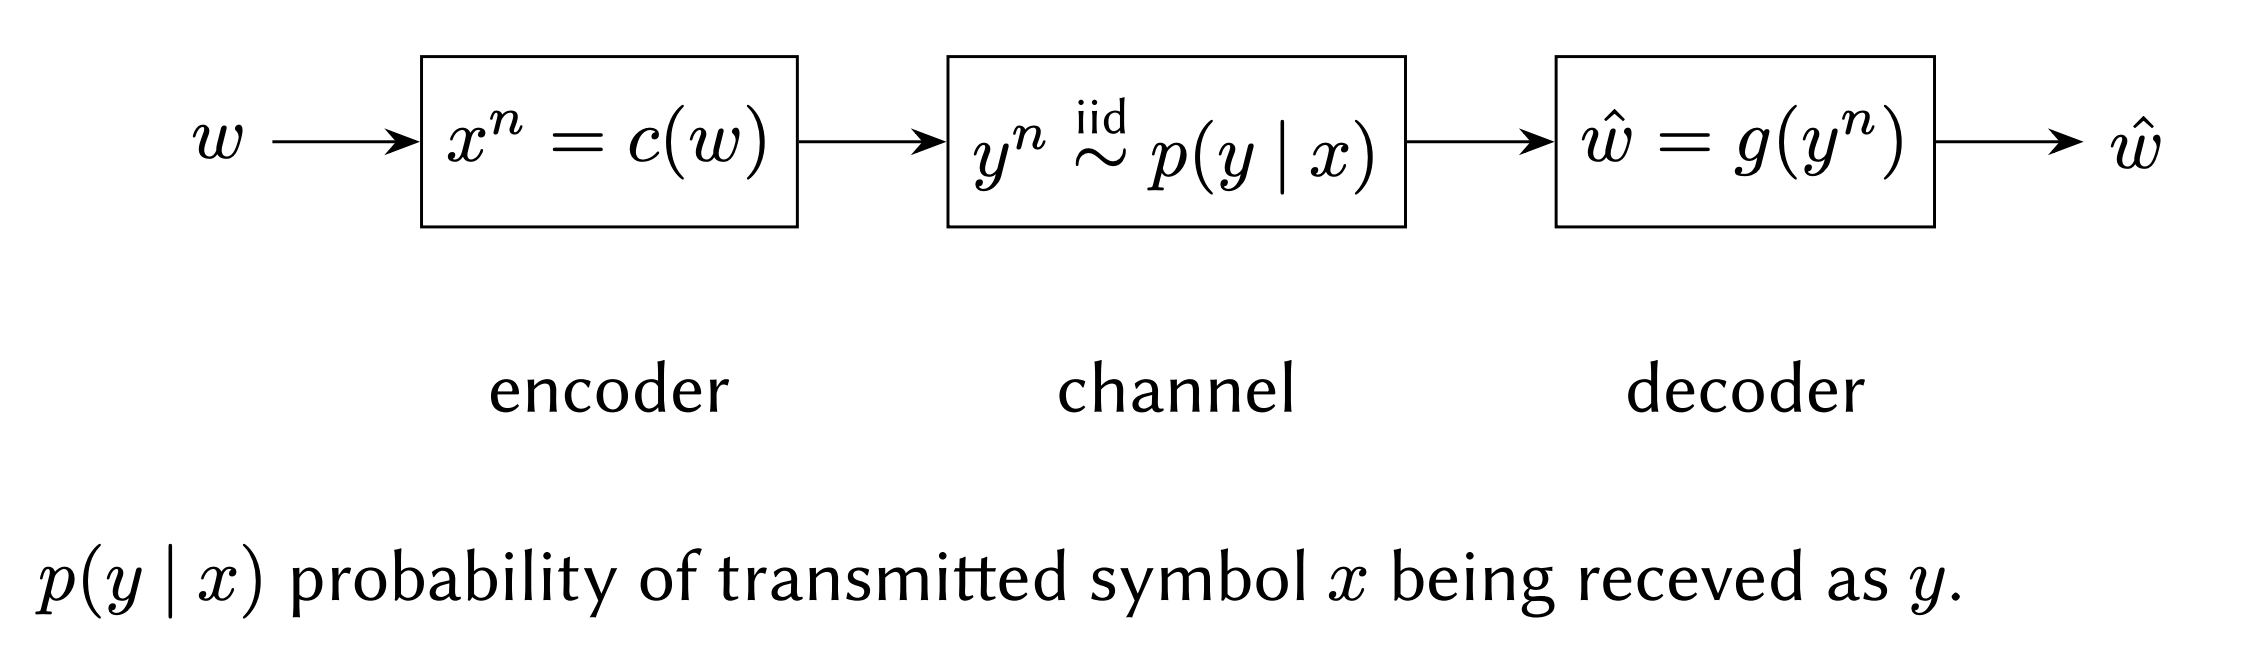
\includegraphics[width=0.75\textwidth]{figures/shannon_pic.png}
\end{center}

\subsection{Important quantities to consider for Schumacher's Compression}

\begin{itemize}
\item \textbf{Entropy Measures:}
For Shannon Entropy \(H(X)\), its analog is \(S(\rho)\).

\item \textbf{Typicality:}
We consider typical subspaces drawn from \(\mathcal{H}\).

\item \textbf{Dimension of Representation:}
Schumacher's typical subspace has dimension \(2^{nS(\rho)}\).

\item \textbf{Compression:}
Schumacher compresses quantum states by projecting them onto the typical subspace using an \textbf{isometry} \(V_{n,\epsilon}\).

\end{itemize}

\section{Quantum Compression - Schumacher's Compression Theorem}

\subsection{Theorem Statement}

\begin{enumerate}

\item Consider a quantum source producing states described by a density matrix \(\rho\), associated with an ensemble \(\{p_i, |\psi_i\rangle\}\) of pure states and probabilities. This acts on a \textit{Complex Euclidean Space} (Hilbert space), with dimension \(d = \dim(\mathcal{H})\). 

\item Direct Part (Achievability): For any rate \(R > S(\rho)\), there exists a sequence of \((n, m, \delta)\)-compression schemes that compress \(\rho^{\otimes n}\) into a subspace of dimension \(2^{nR}\) with perfect fidelity as \(n \to \infty\).
\[
\lim_{n \to \infty} F(D \circ E, \rho^{\otimes n}) = 1,
\]
where \(F(D \circ E, \rho^{\otimes n})\) is the channel fidelity.

\item Converse Part (Optimality): If there exists a sequence of \((n, m, \delta)\)-compression schemes, that compress \(\rho^{\otimes n}\) into subspaces of dimension \(2^{nR}\) with perfect fidelity, then the rate \(R\) must satisfy \(R \geq S(\rho)\).
\[
\lim_{n \to \infty} F(D \circ E, \rho^{\otimes n}) = 1,
\]
then \(R \geq S(\rho)\).

\end{enumerate}

\subsection{Typical Subspaces}
They capture the most probable sequences emitted by the quantum source.

\subsubsection{Definition}

An \(\epsilon\)-typical sequence \((i_1, i_2, \dots, i_n)\) satisfies:
\[
\left| -\frac{1}{n} \log p_{i_1 i_2 \dots i_n} - S(\rho) \right| < \epsilon,
\]
where \(p_{i_1 i_2 \dots i_n} = p_{i_1} p_{i_2} \cdots p_{i_n}\), and \(S(\rho)\) is the von Neumann entropy of \(\rho\):
\[
S(\rho) = - \sum_{i=1}^d p_i \log p_i.
\]

The \(\epsilon\)-typical subspace \(\mathcal{H}_{\text{typ}}\) of \(\mathcal{H}^{\otimes n}\) is the \textit{span} of tensor product states corresponding to \(\epsilon\)-typical sequences of eigenstates \(|\psi_i\rangle\):
\[
\mathcal{H}_{\text{typ}} = \operatorname{span}\left\{ |\psi_{i_1}\rangle \otimes |\psi_{i_2}\rangle \otimes \cdots \otimes |\psi_{i_n}\rangle \, \middle| \, (i_1, i_2, \dots, i_n) \in T_{n, \epsilon}(p) \right\},
\]
where \(T_{n, \epsilon}(p)\) denotes the set of \(\epsilon\)-typical sequences.

\subsubsection{Properties}

\begin{enumerate}
    \item \textbf{High Probability:} The projection of \(\rho^{\otimes n}\) onto \(\mathcal{H}_{\text{typ}}\) captures most of the probability mass:
    \[
    \operatorname{Tr}[\Pi_{n, \epsilon} \rho^{\otimes n}] \geq 1 - \delta_n,
    \]
    only when \(\delta_n \to 0\) as \(n \to \infty\), and \(\Pi_{n, \epsilon}\) is the projector onto \(\mathcal{H}_{\text{typ}}\).

    \item \textbf{Dimension Bound:} The dimension \(D_{\text{typ}} = \operatorname{Tr}[\Pi_{n, \epsilon}]\) of \(\mathcal{H}_{\text{typ}}\) satisfies:
    \[
    D_{\text{typ}} \leq 2^{n(S(\rho) + \epsilon)}.
    \]
    For sufficiently large \(n\) we have:
    \[
    D_{\text{typ}} \geq (1 - \delta_n) 2^{n(S(\rho) - \epsilon)}.
    \]

\item \textbf{Projected State in the Typical Subspace:} 
When $\rho^{\otimes n}$ is projected onto the typical subspace $\mathcal{H}_{\text{typ}}$, it is confined within the subspace: 
\[
\begin{aligned}
    2^{-n(S(\rho) + \epsilon)} \Pi_{n, \epsilon} &\leq \Pi_{n, \epsilon} \rho^{\otimes n} \Pi_{n, \epsilon} \leq 2^{-n(S(\rho) - \epsilon)} \Pi_{n, \epsilon}, \\
    &\implies \rho^{\otimes n} \text{ is approximately uniform within } \mathcal{H}_{\text{typ}}.
\end{aligned}
\]

\end{enumerate}

\begin{center}
    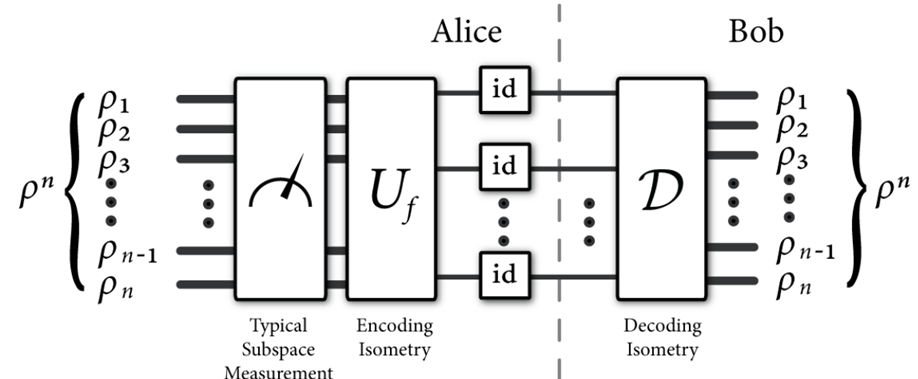
\includegraphics[width=1\textwidth]{figures/schumacher.png}
\end{center}

\subsection{Proof of Schumacher's Compression Theorem}

\subsubsection{Direct Part: Achievability of Compression Rates}

We aim to construct a compression scheme that achieves \textit{asymptotically} perfect fidelity for any rate \(R > S(\rho)\).

\paragraph{Step 1: Typical Projector \(\Pi_{n, \epsilon}\)}

Consider the typical projector \(\Pi_{n, \epsilon}\). It's defined as:
\[
\Pi_{n, \epsilon} = \sum_{(i_1, \dots, i_n) \in T_{n, \epsilon}(p)} |\psi_{i_1} \otimes \cdots \otimes \psi_{i_n}\rangle \langle \psi_{i_1} \otimes \cdots \otimes \psi_{i_n}|,
\]
where \(T_{n, \epsilon}(p)\) is the set of \(\epsilon\)-typical strings of length \(n\), and is based on \(\{p_i\}\) over the basis states \(\{|\psi_i\rangle\}\) of \(\rho\). 
\\
The typical projector maps states into the typical subspace \(\mathcal{H}_{\text{typ}}\), which has the following properties:

\begin{itemize}
    \item \textbf{Dimension Bound:}
    The dimension of the typical subspace is approximately:
    \[
    \dim(\mathcal{H}_{\text{typ}}) \leq 2^{n(S(\rho) + \epsilon)}.
    \]

    \item \textbf{Probability Concentration:}
    The typical subspace captures almost all the probability mass of \(\rho^{\otimes n}\) for sufficiently large n.
    \[
    \text{Tr}[\Pi_{n, \epsilon} \rho^{\otimes n}] \to 1 \quad \text{as } n \to \infty.
    \]

    \item \textbf{Entropy Bound:}
    For any state in the typical subspace, the eigenvalues of \(\rho^{\otimes n}\) satisfy:
    \[
    2^{-n(S(\rho) + \epsilon)} \leq \langle \psi | \rho^{\otimes n} | \psi \rangle \leq 2^{-n(S(\rho) - \epsilon)},
    \]
    where \(|\psi\rangle \in \mathcal{H}_{\text{typ}}\).
\end{itemize}

This subspace represents where most of the information of \(\rho^{\otimes n}\) is present.

\paragraph{Step 2: Encoding and Decoding}

Let \(m_n = \lceil n R \rceil\), where \(R > S(\rho)\). For sufficiently large \(n\), the dimension of the compressed Hilbert space satisfies:
\[
2^{m_n} > 2^{n(S(\rho) + \epsilon)}.
\]

Thus, the typical subspace can be mapped onto a smaller lower-dimensional Hilbert space \((\mathbb{C}^2)^{\otimes m_n}\).

\begin{itemize}
    \item \textbf{Encoding Channel:}
    The encoding map \(E_n : \mathcal{H}^{\otimes n} \to (\mathbb{C}^2)^{\otimes m_n}\) is defined as:
    \[
    E_n(\rho^{\otimes n}) =
    \begin{cases}
        V_{n, \epsilon} \rho^{\otimes n} V_{n, \epsilon}^\dagger, & \text{if } \rho^{\otimes n} \in \mathcal{H}_{\text{typ}}, \\
        |0\rangle \langle 0|, & \text{otherwise}.
    \end{cases}
    \]
    Here, \(V_{n, \epsilon}\) is an \textit{isometry} that maps \(\mathcal{H}_{\text{typ}}\) into \((\mathbb{C}^2)^{\otimes m_n}\). And any state outside the typical subspace is mapped to a fixed state \(|0\rangle \in (\mathbb{C}^2)^{\otimes m_n}\).

    \item \textbf{Decoding Channel:}
    The decoding map \(D_n : (\mathbb{C}^2)^{\otimes m_n} \to \mathcal{H}^{\otimes n}\) is defined as:
    \[
    D_n(Y) = V_{n, \epsilon}^\dagger Y V_{n, \epsilon}.
    \]
This will reconstruct the original state from its compressed representation in the typical subspace, while states outside the typical subspace are mapped to their nearest approximation within  \(\mathcal{H}_{\text{typ}}\).
\end{itemize}

\paragraph{Step 3: Fidelity Analysis}

To analyze the fidelity of the compression scheme, consider the combined operation \(D_n \circ E_n\), represented by its Kraus operators \(\{A_l^{(n)}\}\). The fidelity between the original state \(\rho^{\otimes n}\) and the reconstructed state is given by:
\[
F(D_n \circ E_n, \rho^{\otimes n}) = \left( \sum_{l=1}^{L_n} \left| \operatorname{Tr}(A_l^{(n)} \rho^{\otimes n}) \right| \right)^2.
\]

Using the Cauchy-Schwarz inequality, we can bound the term \(\left| \operatorname{Tr}(A_l^{(n)} \rho^{\otimes n}) \right|\) as:
\[
\left| \operatorname{Tr}(A_l^{(n)} \rho^{\otimes n}) \right|^2 \leq \operatorname{Tr}[\Pi_l^{(n)} \rho^{\otimes n}] \cdot q_l^{(n)},
\]
where:
\[
q_l^{(n)} = \operatorname{Tr}[A_l^{(n)} A_l^{(n)\dagger}] \quad \text{and} \quad \Pi_l^{(n)} = A_l^{(n)\dagger} A_l^{(n)}.
\]

Substituting this back, we bound the fidelity as:
\[
F(D_n \circ E_n, \rho^{\otimes n}) \leq \sum_{l=1}^{L_n} q_l^{(n)} \cdot \operatorname{Tr}[\Pi_l^{(n)} \rho^{\otimes n}].
\]

Since \(D_n \circ E_n\) is a quantum channel, the total probability weights satisfy:
\[
\sum_{l=1}^{L_n} q_l^{(n)} = 1.
\]

For sufficiently large \(n\), the probability mass outside the typical subspace \(\mathcal{H}_{\text{typ}}\) becomes negligible.
\[
\operatorname{Tr}[(I - \Pi_{n, \epsilon}) \rho^{\otimes n}] \to 0 \quad \text{as } n \to \infty.
\]

Thus, the contribution to the fidelity from outside the typical subspace vanishes, ensuring:
\[
F(D_n \circ E_n, \rho^{\otimes n}) \to 1 \quad \text{as } n \to \infty.
\]

\paragraph{Step 4: Achievable Compression Rate}

The dimension of the typical subspace \(\mathcal{H}_{\text{typ}}\) is bounded by:
\[
D_{\text{typ}} \leq 2^{n(S(\rho) + \epsilon)},
\]

To encode the typical subspace, the number of qubits required is:
\[
m_n = \lceil \log_2 D_{\text{typ}} \rceil \leq n(S(\rho) + \epsilon)
\]

The compression rate \(R\), defined as the number of qubits per copy of \(\rho\), is:
\[
R = \lim_{n \to \infty} \frac{m_n}{n}
\]

And finally, from the bound on \(m_n\), it follows that:
\[
R \leq S(\rho) + \epsilon
\]

By choosing \(\epsilon > 0\) arbitrarily small, we ensure that \(R\) can approach \(S(\rho)\). Therefore, for any \(R > S(\rho)\), there exists a sufficiently small \(\epsilon > 0\) such that compression is achievable with asymptotically perfect fidelity.

\subsubsection{Converse Part}
For rates \(R < S(\rho)\), fidelity approaches zero. Assume that there's a sequence of compression schemes with \((n_k, m_k, \delta_k)\) satisfying:
\[
R = \lim_{k \to \infty} \frac{m_k}{n_k} < S(\rho) \quad \text{and} \quad \lim_{k \to \infty} \delta_k = 0.
\]

\begin{flushleft}
Using Kraus decomposition for the channel, fidelity can be bounded:
\end{flushleft}
\[
F(D_k \circ E_k, \rho^{\otimes n_k}) \leq \sqrt{\sum_{l=1}^{L_k} q_l \text{Tr}[\Pi_l \rho^{\otimes n_k}]},
\]

\begin{flushleft}
where \(q_l\) are probabilities associated with the Kraus operators and \(\Pi_l\) are projections with dimensions constrained by the compression rate.
\newline
\newline
The typical subspace of \(\rho^{\otimes n_k}\), which captures almost all of the probability mass, has dimension approximately \(2^{n_k S(\rho)}\). When \(R < S(\rho)\):
\end{flushleft}

\begin{itemize}
    \item The compressed space has dimension \(2^{n_k R}\).
    \item The typical subspace has dimension \(2^{n_k S(\rho)}\).
\end{itemize}

\begin{flushleft}
Since \(R < S(\rho)\), the compressed space (\(2^{n_k R}\)) is exponentially smaller than the typical subspace (\(2^{n_k S(\rho)}\)). This mismatch ensures that the projection operators \(\Pi_l\) cover only a negligible fraction of the typical subspace.
\end{flushleft}

For \(R < S(\rho)\), it follows that:
\[
\begin{aligned}
    \text{Tr}[\Pi_l \rho^{\otimes n_k}] &\to 0 \quad \text{as } k \to \infty, \\
    &\implies F(D_k \circ E_k, \rho^{\otimes n_k}) \to 0.
\end{aligned}
\]
